\documentclass[conference,10pt]{IEEEtran}
%\documentclass[conference,draft,onecolumn]{IEEEtran}
% useful packages, copy and paste from diff sources

\usepackage[english]{babel}
\usepackage[T1]{fontenc}
\usepackage{cite,url,color} % Citation numbers being automatically sorted and properly "compressed/ranged".
\usepackage{graphics,amsfonts}
\usepackage{epstopdf}
\usepackage[pdftex]{graphicx}
\usepackage[cmex10]{amsmath}
% Also, note that the amsmath package sets \interdisplaylinepenalty to 10000
% thus preventing page breaks from occurring within multiline equations. Use:
\interdisplaylinepenalty=2500
% after loading amsmath to restore such page breaks as IEEEtran.cls normally does.
\usepackage[utf8]{inputenc}
% Useful for displaying quotations
%\usepackage{csquotes}
% Compact lists
%\let\labelindent\relax
\usepackage{enumitem}

%tikz figures
\usepackage{tikz}
\usetikzlibrary{automata,positioning,chains,shapes,arrows}
\usepackage{pgfplots}
\usetikzlibrary{plotmarks}
\newlength\fheight
\newlength\fwidth
\pgfplotsset{compat=newest}
\pgfplotsset{plot coordinates/math parser=false}

\usepackage{array}
% http://www.ctan.org/tex-archive/macros/latex/required/tools/
%\usepackage{mdwmath}
%\usepackage{mdwtab}
%mdwtab.sty	-- A complete ground-up rewrite of LaTeX's `tabular' and  `array' environments.  Has lots of advantages over
%		   the standard version, and over the version in `array.sty'.
% *** SUBFIGURE PACKAGES ***
%\usepackage[tight,footnotesize]{subfigure}
\usepackage{subfig}

\usepackage[top=1.5cm, bottom=2cm, right=1.6cm,left=1.6cm]{geometry}
\usepackage{indentfirst}

\usepackage{times}
% make sections titles smaller to save space
%\usepackage{sectsty}
%\sectionfont{\large}
% enable the use of 'compactitem', a smaller 'itemize'
%\usepackage{paralist}

% MP
% to split equations using dmath env
\usepackage{breqn}
% nice rules in tables
\usepackage{booktabs}

%\setlength\parindent{0pt}
\linespread{1}

% MC
\newcommand{\MC}[1]{\textit{\color{red}MC says: #1}}
\newcommand{\AZ}[1]{\textit{\color{blue}AZ says: #1}}
\newcommand{\MP}[1]{\textit{\color{green}MP says: #1}}

\usepackage{placeins}


%%%%%%%%%%%%%%%%%%%%%%%%%%%%%%%%%%%%%%%%%%
\begin{document}
%%%%%%%%%%%%%%%%%%%%%%%%%%%%%%%%%%%%%%%%%%
\title{V2X connectivity with real velocity traces}

\author{\IEEEauthorblockN{Luca della Libera, Andrea Rossi, Jacopo Pegoraro}
\IEEEauthorblockA{Department of Information Engineering, University of Padova -- Via Gradenigo, 6/b, 35131 Padova, Italy\\Email: {\tt\{luca.dellalibera.1, andrea.rossi.26, jacopo.pegoraro\}@studenti.unipd.it}
}}

\maketitle

\begin{abstract}
The millimiter waves bands offer the opportunity to exceptionally increase the data rates for fifth-generation cellular systems and support the birth of emerging automative applications. The performance of end-to-end communicanications dramatically decrease when there are obstacles in the line of sight (LOS) between a base station and an user equipment.
This paper analyze the performance of well-known protocol (e.g. UDP) in realistic urban automative scenario, under different handover policies, based on the real-world traffic data simulation of the mobility of cars in SUMO (an open source simulator which allows modeling traffic systems, including road vehicles) and imported in another network simulation platform like ns3. In future urban scenario, important information like the route of a car from from a starting point to a destination could be useful to predict which cell is more suitable to ensure a better connection. We show that these policies, combinaned with prior knownledge of the scenario, can improve the throughput and/or delay of the connection.
\end{abstract}

%%%%%%%%%%%%%%%%%%%%%%%%%%%%%%%%%%%%%%%%%
\section{Introduction}\label{sec:intro}
%%%%%%%%%%%%%%%%%%%%%%%%%%%%%%%%%%%%%%%%%

In the last few years a vast number of automotive applications were developed and many of them are already being tested on the latest generation vehicles: self-driving cars, sensors for real time object recognition and infotainment are only some examples. However, a fundamental requirement to effectively implement these applications is to have high data rates communication capabilities as the sensors and devices required could produce data in the order of magnitude of hundreds of Mb/s \cite{surveh}.
The state of the art protocol for communication in a vehicular environment is the \emph{dedicated short-range communication} (DSRC) that, however, cannot satisfy the mentioned requirements, having a theoretical rate of 27Mb/s \cite{surveh}. For this reason there is growing interest in the potential of millimiter wave technologies, that make use of the frequency spectrum over 10 GHz providing data rates in the order of the Gb/s. These transmission capabilities can be achieved using carriers at very high frequency, therefore increasing the available bandwidth that could be exploited and consequently the capacity of the radio links. However there are some drawbacks of this approach that become even more significant in outdoor and vehicular situations, one is the high attenuation that mmWave signals are subject to, indeed the \emph{path-loss} in a radio channel depends on the reciprocal square-root of the wavelength $\lambda$, so reducing $\lambda$ (increasing frequency) the path-loss increases, thus there is need for more mmWave base stations to avoid lack of coverage. Another problem is that to avoid the just mentioned high attenuation, massive MIMO is used to convey the signal into narrow directional beams instead of the isotropic transmission used in the present standards, so when facing with a high speed nodes scenario as can be a vehicular one, mmWave technologies can perform poorly due to blockage and bad beam aligning \cite{mmvehicle}.

To partially solve these problems in a future urban scenario with high density of mmWave base stations we can work on improving the \emph{handover} procedure, that is the method used to control the switch of nodes between different base stations as they move in the scenario. The current handover procedure used in mmWave networks is the one inherited from the 4G-LTE standard and is based on connecting to the station that provides the maximum received SINR among those that are reachable. In this paper we reproduced a typical urban scenario with the help of SUMO, a urban mobility simulator that allows to export the mobility traces from the simulation into a network simulator such as ns-3. The scenario is that of a crossroad with traffic lights regulating the flow of 12 cars and is described in more detail in the next sections. Using ns-3 and the mobility traces we simulated a mmWave network with 3 base stations at the sides of the road and 12 nodes (the cars) passing through the crossroad and continuously receiving UDP packets from the base stations. Starting from this simulation environment we tried 4 different handover procedures, beginning with the standard one and then seeing if slight modifications like using a SINR threshold or maximizing the channel capacity could lead to some improvements in terms of throughput or delay. 




%%%%%%%%%%%%%%%%%%%%%%%%%%%%%%%%%%%%%%%%%%%%
\section{Related Work}\label{sec:sota}
%%%%%%%%%%%%%%%%%%%%%%%%%%%%%%%%%%%%%%%%%%%%
The interest for millimiter waves bands, between 30 and 300 GHz, where the avaiable bandwidths are much wider than today's cellular networks is growing more and more, but there is a fear that the propagation of millimeter waves signals is much less favorable: these signals suffer from severe shadowing and intermittent connectivity \cite{mmwwicom} \cite{mmwcomsy}. Many researchs has been conducted for analizing the challenges and opportunities at different layers of the protocol stack that millimeter can give to support the massive demand for high data rates that is expected to be required in next generation of automotive applications.
Rangan et al. \cite{mmwpac} analyze various technologies including adaptive beamforming, multihop relaying, heterogeneous network architectures, and carrier aggregation used in the millimeter wave context, highlighting that this systems can offer at least an order of magnitude in capacity over current state-of-the-art LTE systems, at least for outdoor covarage.

Regarding highly dense or highly mobile vehicular scarnarios, Giordani et al. \cite{mmvehicle} observe that for these scenarios, vehicles are subject to frequent handover and obstacle can expose to risk a successfull communication even if the automative nodes are perfectly aligned, since millimeter waves cannot penetrate through solid materials. Moreover beam alignment can be favored by known geographical position at least to limit the search area of the most favorable beam direction. Anyway, based on their analysis, the permonance of the automative nodes strictly depends on the specific environment in which the vehicles are deployed, and must consider the number of the nodes, the vehicle's speed and the beam tracking periodicity.

To better capture the most significant aspects of the millimeter wave in vehicular networks  New York University and the University of Padova developed an open-source millimeter wave simultation tool for LTE-like 5G mmWave cellulare networks, which can be used to evaluate the perfomarce of an end-to-end communication. This was developed as new module within the largely used ns-3 network simulator, based on LTE architecture. Mezzavilla et al. \cite{e2esim} propose a tutorial of this new module and the initial setting information of the layers of the protocol stack which has been used in our research project to analyze the performance of the throughput and the delay of an end-to-end communication, under different handover policies, in an high-mobility scenario, expanding the code of this module.

Another interesting work based on the improvement of the performance of a millimeter wave communication has been proposed by Polese et al. \cite{imphand} with the study of dual connectivity. One of the main tools to improve the robustness of millimeter wave systems is multi-connectivity: maintaining connections to multiple cells (both 5G mmWave cells and/or 	common 4G cells), the user can find alternate routes to keep the connection.
Based on their observations and results, our model maintain the dual connectivity option through the possibility to connect vehicles to a LTE cell in order to make the connection more robust, even if it is used only if all 5G mmWave cells are in outage.

In this paper we aim to evaluate the performance of vehicles' connection in a realistic urban automotive scenario, characterize by real-world traffic data in a crossroad with a traffic light in which many vehicles remain connected to the same cell for a while, with the presence of obstacles like trees and buildings which can decrease the Signal to Interference plus Noise Ratio (SINR) of the connection, investigating in better policies of handover.
In the next sections we present in detail our model and our handover policies used, highlighting the most relevant results of the simulation.



%%%%%%%%%%%%%%%%%%%%%%%%%%%%%%%%%%%%%%
\section{System Model}\label{sec:symo}
%%%%%%%%%%%%%%%%%%%%%%%%%%%%%%%%%%%%%%
The System model is a description of your operating assumptions with related motivation and justification

%%%%%%%%%%%%%%%%%%%%%%%%%%%%%%%%%%%%%%%%%%%%%%%
\section{Results}\label{sec:res}
%%%%%%%%%%%%%%%%%%%%%%%%%%%%%%%%%%%%%%%%%%%%%%%
We compare the default handover policy (DHO) in used in the ns3 LTE-like 5G mmWave module as 
described below, in which an user equipment perform an handover from a base station to another when the new base station has a better SINR for a prefixed interval of time. Figure 1 show a typical behavior of the SINR curve for a vehicle respect to all base stations in our urban scenario. The instants of time in which a vehicle connects from a base station to another is highlighted. The errors in the channel and non-line-of-sight (NLOS) between the automotive car and the cell causes the irregular trend of the lines. Moreover Figure 2 shows the behavior of the two of the metrics used to compare the performance of our simulations: the throughput and the delay of the transmission during the entire period in which the vehicles are crossing the roads, with particular attention to their mean values.

\begin{figure*}[h]
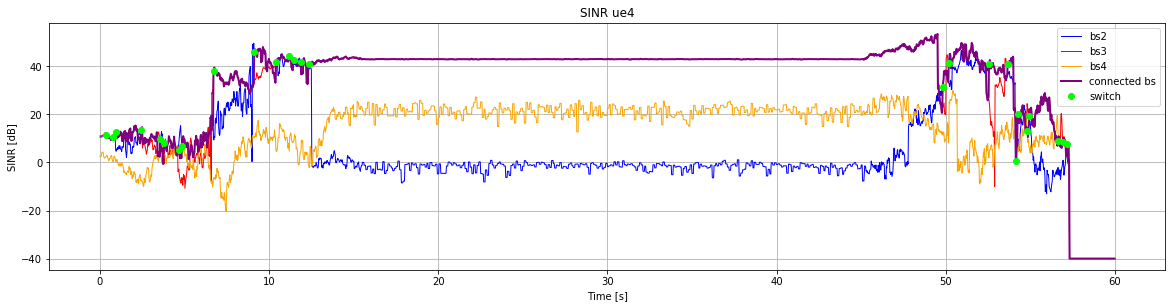
\includegraphics[scale=0.4]{ue4_switch_dho.png}
\caption{SINR of a vehicle in the road with points of switch}
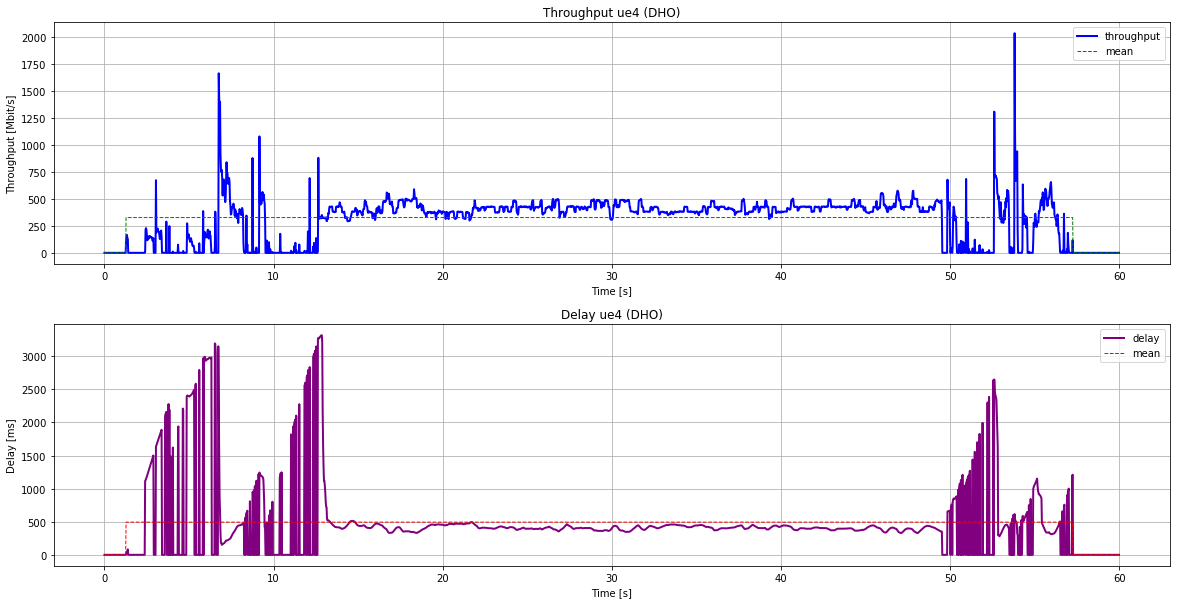
\includegraphics[scale=0.4]{ue4_td_dho.png}
\caption{Throughput and delay of a vehicle in the road}
\end{figure*}

The total amount of traffic generated by vehicles during 60 seconds simulation has been obtained adding the throughput and the delay of each user in the scenario. A graphic result is shown in Figure 3.
\begin{figure*}[h]
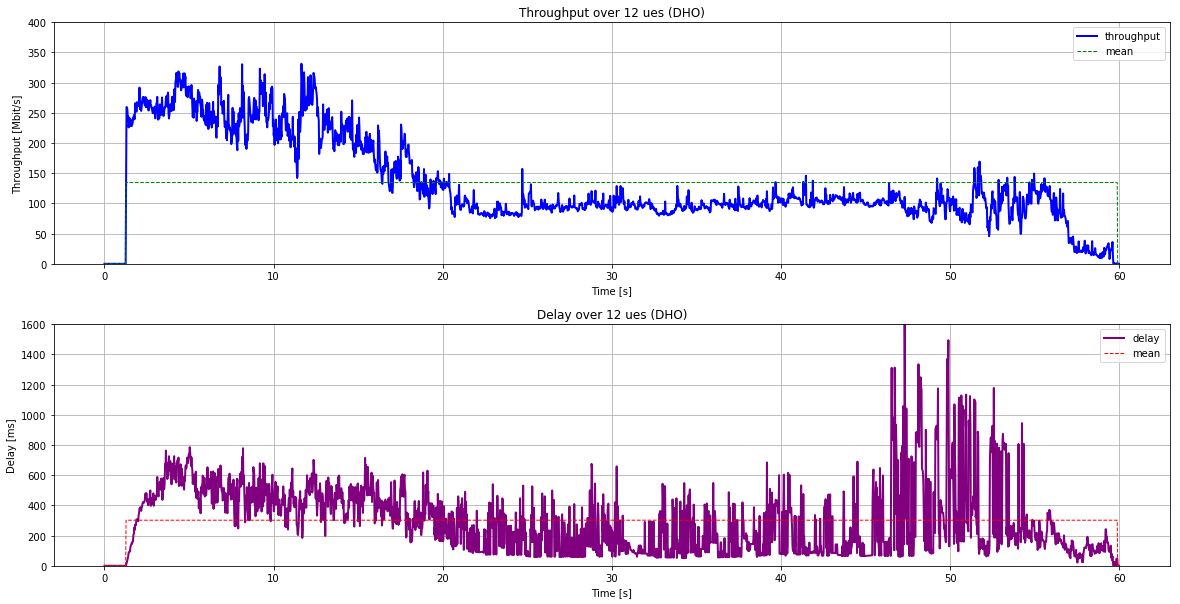
\includegraphics[scale=0.4]{results_dho.png}
\caption{Total throughput and delay of DHO handover policy}
\end{figure*}

Now we want to compare the results obtained performing the three different handover policy described in the previous section.
Figures 4, 5 and 6 represent respectively the total throughput generated during the simulation and the delay of three different policies: 
\begin{itemize}
\item the first is \textit{MHO_100} in which the handover is made when the difference of the SINR between the current base station and the target cell is more than a constant fixed at 100 (in linear scale)
\item the second policy is \textit{MHO_mean} in which the handover is made based on the threshold which depends on the mean of the different SINR of the base station in the scenario
\item the third method is \textit{MHO_Shannon} in which the handover condition is based on the Shannon's theorem for the channel capacity and the handover happens when the capacity of the channel on the target cell is higher than the current. 
\end{itemize}
\
\begin{figure*}[h]
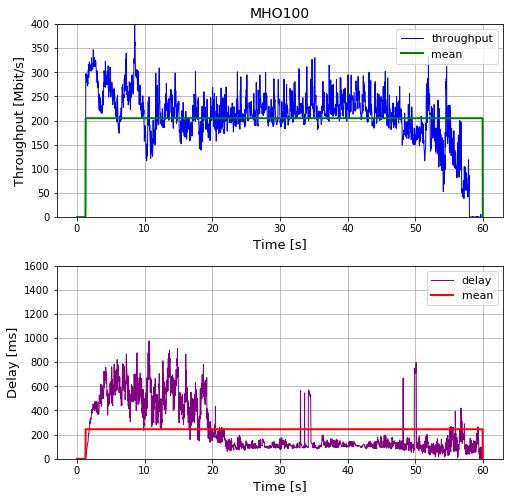
\includegraphics[scale=0.4]{results_mho_100.png}
\caption{Total throughput and delay of MHO_100 handover policy}
\end{figure*}
\begin{figure*}[h]
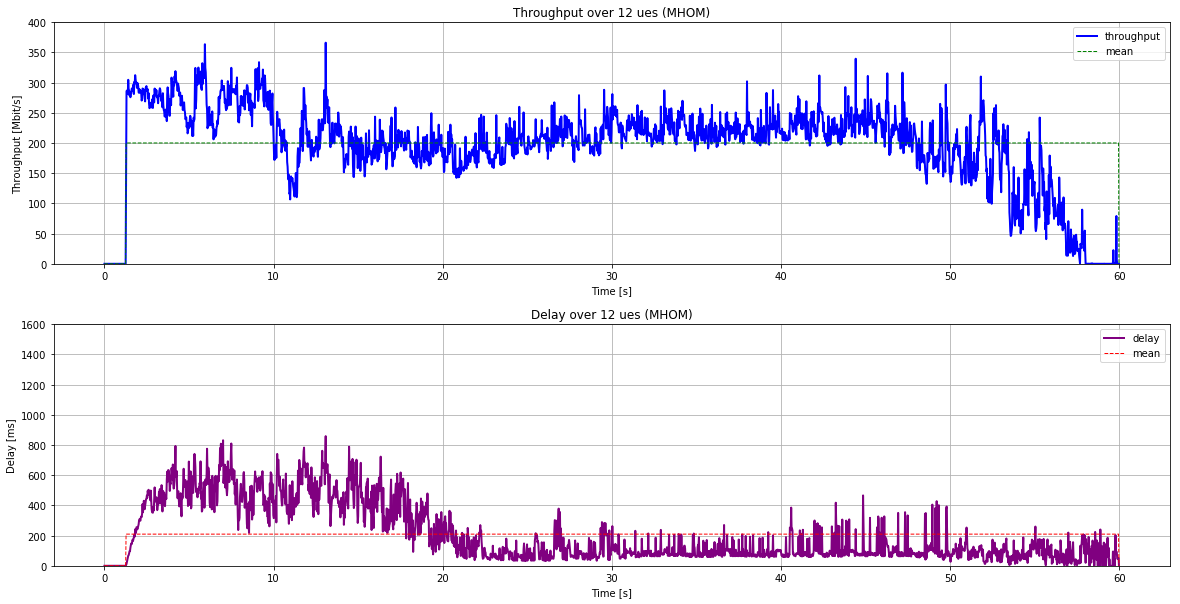
\includegraphics[scale=0.4]{results_mho_mean.png}
\caption{Total throughput and delay of MHO_mean handover policy}
\end{figure*}
\begin{figure*}[h]
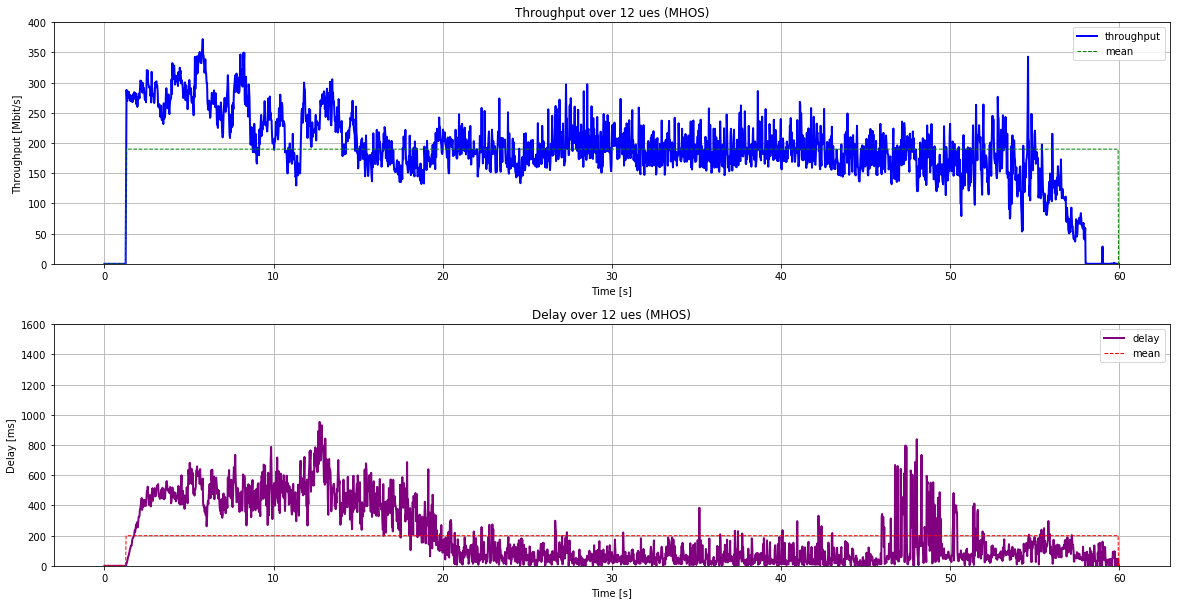
\includegraphics[scale=0.4]{results_mho_shannon.png}
\caption{Total throughput and delay of MHO_Shannon handover policy}
\end{figure*}
As we can see in the plots each policy reach similar mean values for throughput and delay and in each of these cases the differences with the default policy are appreciable. Each method reach an improvement of about 25\% for the mean throughput, while regarding the delay, its mean reaches a decrease of about 30\%, with small differences between  Anyway, among the proposed policies, \textit{MHO_100} reaches the best mean throughput but the worst mean delay and so it is needed a trade off between these two metrics.
The comparison between the three policies with respect to default one is shown in Figure 7.
\begin{figure*}[h]
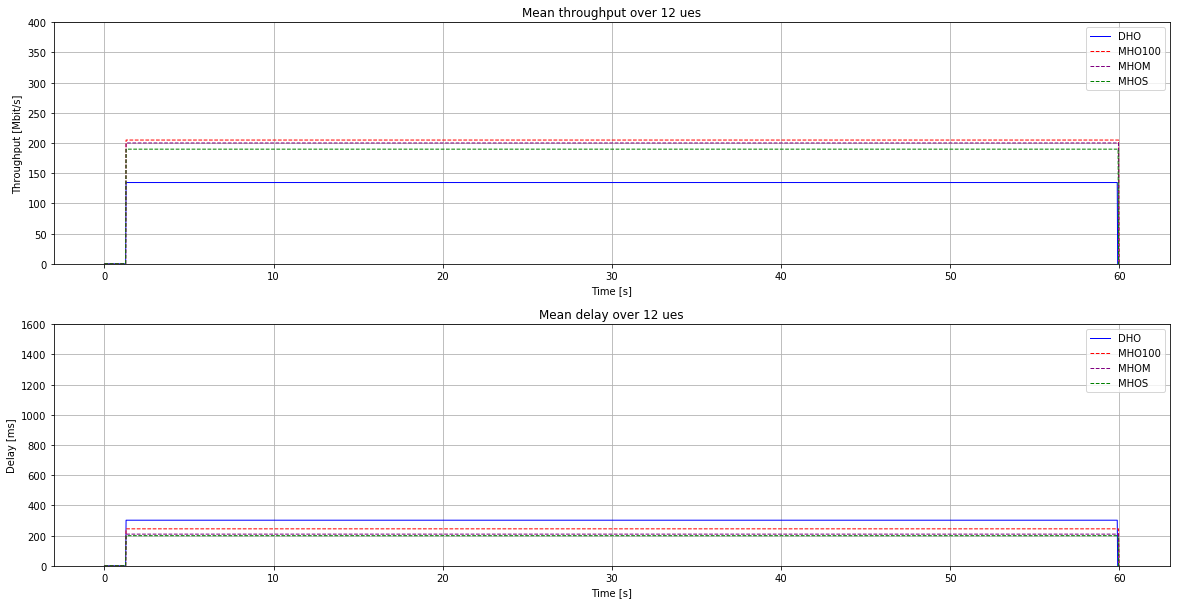
\includegraphics[scale=0.4]{results.png}
\caption{Comparison between four analyzed policies}
\end{figure*}
Another result which has to be compared among this differet methods is the number of the handover which occurs during the simulation. Figure 8 shows that ...

As part of the future work on this research project, we aim to give more randomness to the scenario for example the random choiche of the building, the presence of pedastrians in the street or change the croassroad shape, increasing the number the avaiable directions and the vehicles. Anyway the randomness of our scenario is perfomed by the variability of the channel's charateristics and the size of the sent packets.
%%%%%%%%%%%%%%%%%%%%%%%%%%%%%%%%%%%
\section{Conclusions}\label{sec:conclusion}
%%%%%%%%%%%%%%%%%%%%%%%%%%%%%%%%%%%
Conclusions are a superbrief summary of what has been done and highlighting of the "take home message"



\addtocontents{toc}{Bibliografia}
\begin{thebibliography}{15}
	
	\bibitem{surveh}
	V. Va, T. Shimizu, G. Bansal, R. W. Wealth Jr et al.,
	\textit{Millimiter Wave vehicular communications: a survey}. 
	Foundations and trends in Networking, vol. 10, no. 1, 2016..
	
	\bibitem{mmvehicle}
	M. Giordani, A. Zanella, M. Zorzi,
	\textit{Millimiter Wave Communication in Vehicuar Networks: Challenges and Opportunities}. 
	IEEE 6th International Conference on Modern Circuits and System Technologies, 2017.
	
	\bibitem{imphand}
	M. Polese, M. Giordani, M. Mezzavilla, S. Rangan, M. Zorzi,
	\textit{Improved Handover Through Dual Connectivity in 5G mmWave Mobile Networks}. 
	IEEE Journal on Selected Areas in Communications, vol. 35, no. 9, pp. 2069-2084, 2017.
	
	\bibitem{e2esim}
	M. Mezzavilla, M. Zhang, M. Polese, R. Ford, S. Dutta, S. Rangan, M. Zorzi,
	\textit{End-to-End Simulation of 5G mmWave Networks}. 
	arXiv preprint, 2017.
	
	\bibitem{mmwwicom}
	T. S. Rapparport, R. W: Heath Jr, R. C. Daniels, J.N. Murdock,
	\textit{Millimeter Wave Wireless communications}.
	Prentice Hall, 2015.
	
	\bibitem{mmwcomsy}
	K. C. Huang, P. Rapajic, Z. Wang
	\textit{Millimiter Wave Communication Systems}.
	Wiley, 2011.
	
	\bibitem{mmwpac}
	S. Rangan, T. S. Rappaport, E. Erkip,
	\textit{Millimiter-Wave Cellular Wireless Netwoeks: Potentials and Challenges}
	Proceedings of the IEEE, vol. 102, no. 3, March 2014
	
	
	
\end{thebibliography}



\end{document}
